\documentclass[a4paper,11pt]{article}

\usepackage{../préambule}

\newmdenv[style=coursstyle]{attention}

\begin{document}

{\tiny colle dans ton cahier d'exercices}

\begin{exercice*}[3]
	Fait le symétrique de la figure suivante par rapport à l'axe $(d)$ :

	\newcommand{\sqrttwo}{\directlua{tex.print(math.sqrt(2))}}
	\newcommand{\timessqrttwo}[1]{\directlua{tex.print(math.sqrt(2) * tonumber(#1))}}

	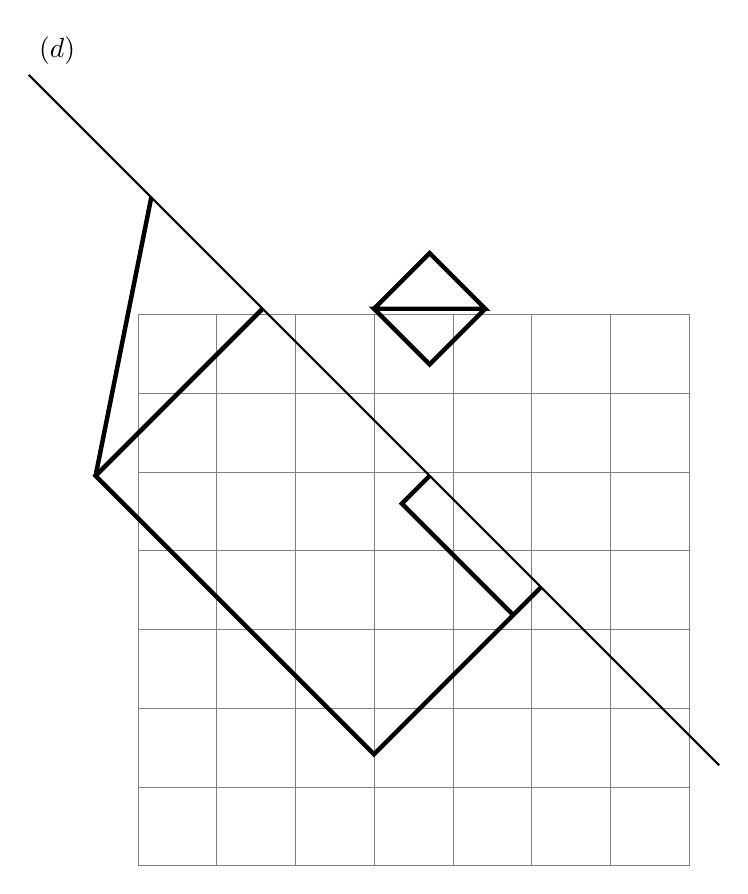
\begin{tikzpicture}[scale=1]
		\draw[step=\sqrttwo,gray,ultra thin] (\timessqrttwo{-3},\timessqrttwo{0}) grid ++(\timessqrttwo{7},\timessqrttwo{7});
		\draw[black,thick,rotate=45] (4,-2.2) -- (4,10.2) node[anchor=south west]{$(d)$};

		\draw[black,ultra thick,rotate=45] (4,1) -- ++(-3,0) -- ++(0,5) -- ++(3,0);
		\draw[black,ultra thick,rotate=45] (4,8) -- ++(-3,-2);
		\draw[black,ultra thick,rotate=45] (3.5,1) -- ++(0,2) -- ++(0.5,0);
		\draw[black,ultra thick,rotate=45] (6,4) -- ++(-1,0) -- ++(0,1) -- ++(1,-1) -- ++(0,1) -- ++(-1,0);
	\end{tikzpicture}

	Quelle figure obtient-on ?
\end{exercice*}

\vspace{2em}
\hrule
\vspace{1em}

{\tiny colle dans ton cahier d'exercices}

\begin{exercice*}[3]
	Fait le symétrique de la figure suivante par rapport à l'axe $(d)$ :

	\newcommand{\sqrttwo}{\directlua{tex.print(math.sqrt(2))}}
	\newcommand{\timessqrttwo}[1]{\directlua{tex.print(math.sqrt(2) * tonumber(#1))}}

	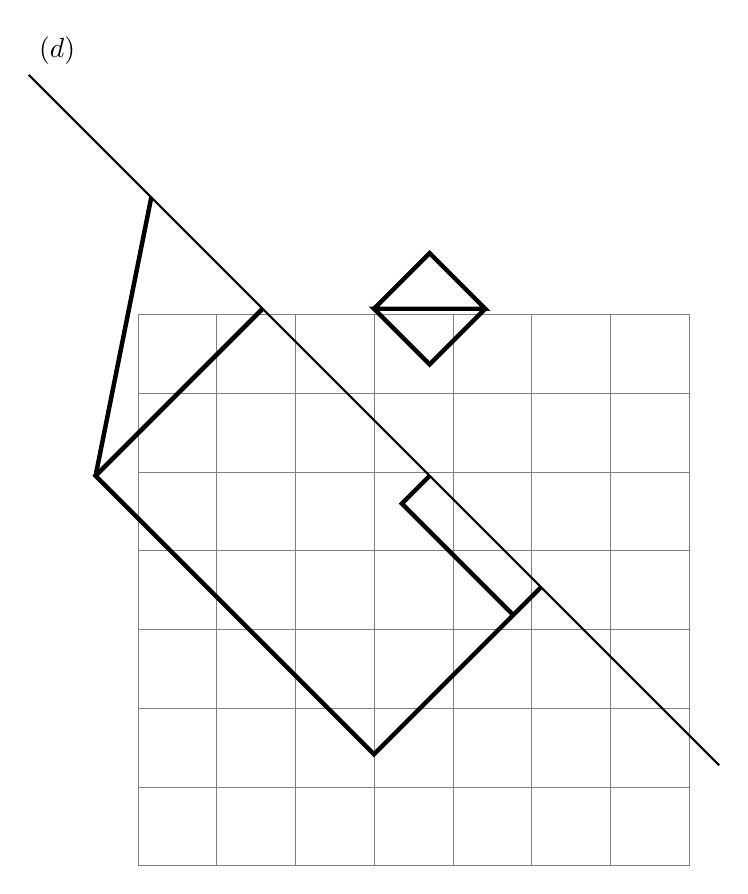
\begin{tikzpicture}[scale=1]
		\draw[step=\sqrttwo,gray,ultra thin] (\timessqrttwo{-3},\timessqrttwo{0}) grid ++(\timessqrttwo{7},\timessqrttwo{7});
		\draw[black,thick,rotate=45] (4,-2.2) -- (4,10.2) node[anchor=south west]{$(d)$};

		\draw[black,ultra thick,rotate=45] (4,1) -- ++(-3,0) -- ++(0,5) -- ++(3,0);
		\draw[black,ultra thick,rotate=45] (4,8) -- ++(-3,-2);
		\draw[black,ultra thick,rotate=45] (3.5,1) -- ++(0,2) -- ++(0.5,0);
		\draw[black,ultra thick,rotate=45] (6,4) -- ++(-1,0) -- ++(0,1) -- ++(1,-1) -- ++(0,1) -- ++(-1,0);
	\end{tikzpicture}

	Quelle figure obtient-on ?
\end{exercice*}

\end{document}